\documentclass[varwidth=true, border=2pt]{standalone}
\usepackage{tikz}
\usetikzlibrary{patterns}

\begin{document}
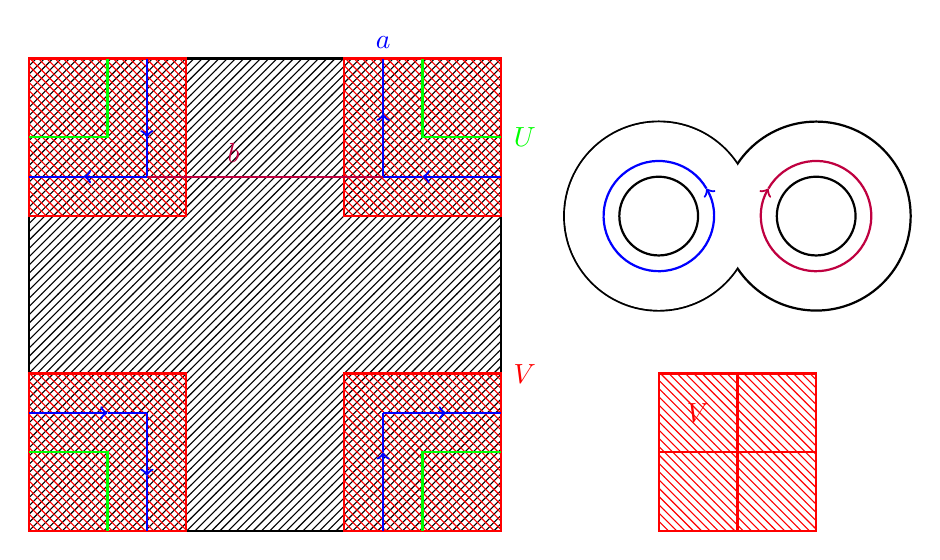
\begin{tikzpicture}[thick]
    \draw[pattern=north east lines] (-3,3) -- (3,3) -- (3,-3) -- (-3,-3) -- cycle;
    \begin{scope}
        \draw[red, pattern color=red, pattern=north west lines] (-3,-1) -- (-1,-1) -- (-1,-3) -- (-3,-3) -- cycle;
        \draw[->,blue] (-3,-1.5) -- (-2,-1.5);
        \draw[blue] (-2,-1.5) -- (-1.5,-1.5);
        \draw[->,blue] (-1.5,-1.5) -- (-1.5,-2.3);
        \draw[blue] (-1.5, -2.3) -- (-1.5, -3);
        \draw[green] (-3,-2) -- (-2,-2) -- (-2, -3);
    \end{scope}
    \begin{scope}[rotate=90]
        \draw[red, pattern color=red, pattern=north west lines] (-3,-1) -- (-1,-1) -- (-1,-3) -- (-3,-3) -- cycle;
        \draw[->,blue] (-3,-1.5) -- (-2,-1.5);
        \draw[blue] (-2,-1.5) -- (-1.5,-1.5);
        \draw[->,blue] (-1.5,-1.5) -- (-1.5,-2.3);
        \draw[blue] (-1.5, -2.3) -- (-1.5, -3);
        \draw[green] (-3,-2) -- (-2,-2) -- (-2, -3);
    \end{scope}
    \begin{scope}[rotate=180]
        \draw[red, pattern color=red, pattern=north west lines] (-3,-1) -- (-1,-1) -- (-1,-3) -- (-3,-3) -- cycle;
        \draw[->,blue] (-3,-1.5) -- (-2,-1.5);
        \draw[blue] (-2,-1.5) -- (-1.5,-1.5);
        \draw[->,blue] (-1.5,-1.5) -- (-1.5,-2.3);
        \draw[blue] (-1.5, -2.3) -- (-1.5, -3);
        \draw[green] (-3,-2) -- (-2,-2) -- (-2, -3);
    \end{scope}
    \begin{scope}[rotate=270]
        \draw[red, pattern color=red, pattern=north west lines] (-3,-1) -- (-1,-1) -- (-1,-3) -- (-3,-3) -- cycle;
        \draw[->,blue] (-3,-1.5) -- (-2,-1.5);
        \draw[blue] (-2,-1.5) -- (-1.5,-1.5);
        \draw[->,blue] (-1.5,-1.5) -- (-1.5,-2.3);
        \draw[blue] (-1.5, -2.3) -- (-1.5, -3);
        \draw[green] (-3,-2) -- (-2,-2) -- (-2, -3);
    \end{scope}

    \node[red]    at (3.3,-1) {$V$};
    \node[green]  at (3.3,2) {$U$};
    \node[blue]   at (1.5, 3.2) {$a$};
    \node[purple] at (-0.4, 1.8) {$b$};
    \draw[purple] (-1.5,1.5) -- (1.5,1.5);

    \begin{scope}[xshift=6cm, yshift=-2cm]
        \node[red] at (-0.5,0.5) {$V$};
        \draw[red,pattern color=red, pattern=north west lines] (-1,1) -- (1,1) -- (1,-1) -- (-1,-1) -- cycle;
        \draw[red] (-1,0) -- (1,0);
        \draw[red] (0,-1) -- (0,1);
    \end{scope}

    \node[blue]   at (4.5, 1.7) {$a$};
    \node[purple] at (7.5, 1.7) {$b$};
    \begin{scope}[xshift=5cm, yshift=1cm]
        \draw[black,fill=white]   (0,0) circle(1.2cm);
        \draw[black, fill=white]   (2,0) circle(1.2cm);
        \path[fill=white]   (0,0) circle(1.19cm);
        \draw[black]  (0,0) circle(0.5cm);
        \draw[black]  (2,0) circle(0.5cm);
        \draw[blue,->]   (0,0)+(30:0.7cm) arc (30:390:0.7cm);
        \draw[purple,<-] (2,0)+(150:0.7cm) arc (150:510:0.7cm);
    \end{scope}
\end{tikzpicture}
\end{document}
